\chapter{Continuous Random Variables}

In this chapter, we assume that a probability space $(S, \mathcal{A}, P)$ is given.

\section{Distribution Function}

\begin{example}
Let $X$ be a discrete random variable with $\im X = \{ 0, 1, 2, 3, 4, 5 \}$ and let $p_X$ be its probability mass function given by $p_X (x) = 1/6$, if $x = 0, 1, 2, 3, 4, 5$.
    \begin{enumerate}[label=\alph*)]
        \item What is $P (X \leq -1 )$?
        \item What is $P (X \leq 2 )$?
        \item What is $P (X \leq 3.5 )$?
    \end{enumerate}
\end{example}
\begin{sol*}
\begin{enumerate}[label=\alph*)]
    \item Since $X$ takes only non-negative values, $\{ X \leq -1 \} = \varnothing$ and therefore $P (X \leq -1) = 0$.
    \item We have
        \[
            P (X \leq 2) = P (X = 0) + P (X = 1) + P (X = 2) = p_X (0) + p_X (1) + p_X (2) = \frac{3}{6} = \frac{1}{2} .
        \]
    \item We have 
        \[
            P (X \leq 3.5 ) = P (X = 0) + P (X = 1) + P (X = 2) + P (X = 3) = \frac{4}{6} = \frac{2}{3} .
        \]
\end{enumerate}
\end{sol*}

In the case of a discrete random variable, from Problem \ref{P:EquivalentEvents}, we know that $\{ X \leq x \}$ is an event, whenever $x \in \mR$. To include more random variable where $\im X$ is not necessarily discrete, we will have to require that $\{X \leq x \}$ is measurable because we will be interested in this event rather that $\{ X = x \}$. 

\begin{definition}
A map $X : S \ra \mR$ is a random variable if $\{ X \leq x \}$ is an event, for every $x \in \mR$.
\end{definition}

\underline{\textbf{Note:}} From Problem \ref{P:EquivalentEvents}, when $\im X$ is discrete, then this above definition also describes the discrete random variables.

\begin{definition}
If $X$ is a random variable, the \underline{distribution function} of $X$ is the function $F_X : \mR \ra [0,1]$ defined by
\[
    F_X (x) = P (X \leq x ) .
\]
\end{definition}

\begin{example}\label{Ex:DistributionFunction}
Three coins are flipped and let $X$ be the number of heads obtained. We know that $P (X = 0) = 1/8$, $P (X = 1) = P (X = 2) = 3/8$, and $P (X = 3) = 1/8$. Find the distribution function of $X$.
\end{example}

\begin{sol*}
Let $\lfloor x \rfloor$ be the larger integer smaller than $x$. For example $\lfloor 3.5 \rfloor = 3$ and $\lfloor -4.5 \rfloor = -5$.

When $x < 0$, then $F_X (x) = P (X \leq x ) = 0$. For $x \geq 0$, we get
    \[
        F_X (x) = \sum_{k = 0}^{\lfloor x \rfloor} p_X (k) .
    \]
The graph is illustrated in the Figure \ref{fig:DistributionFromFirstExample}. \hfill $\triangle$
\end{sol*}
\begin{figure}[ht]
\centering
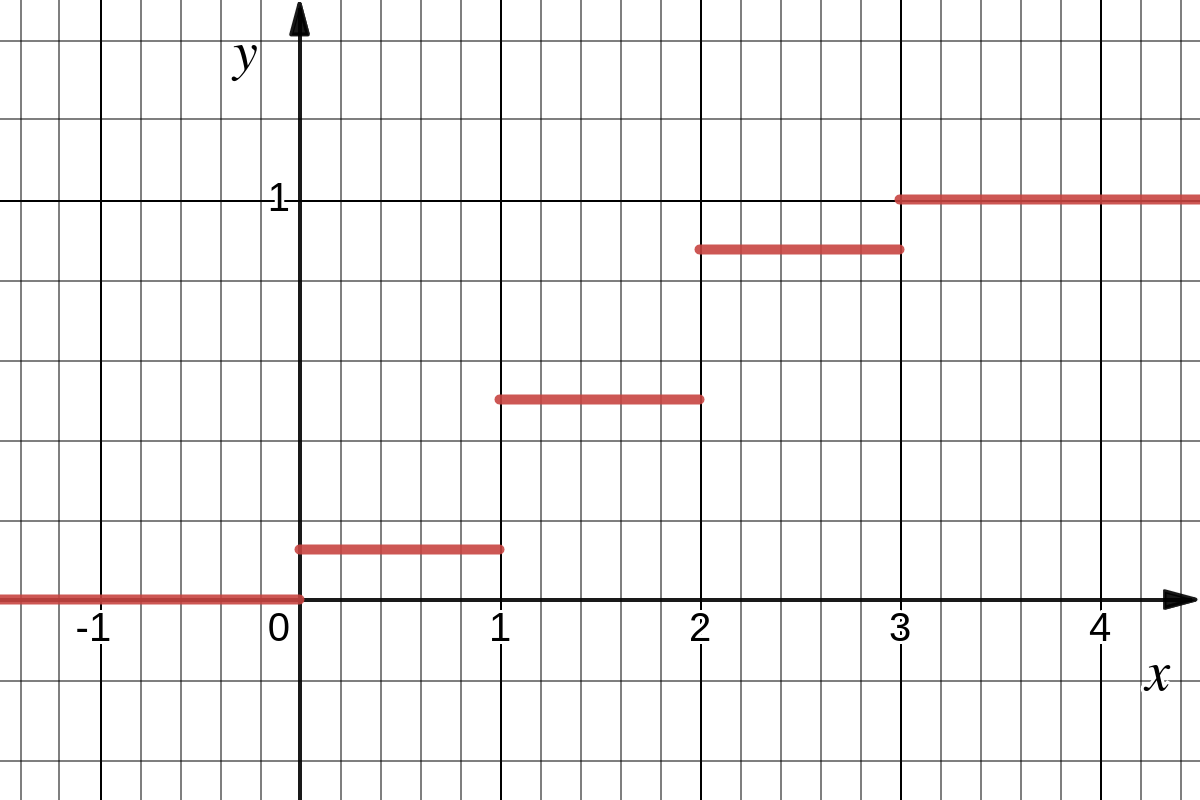
\includegraphics[scale=0.3]{distributionFunction-Example.png}
\caption{Distribution function from Example \ref{Ex:DistributionFunction}}\label{fig:DistributionFromFirstExample}
\end{figure}

\begin{theorem}
Let $X$ be a random variable. Then its distribution function $F_X$ satisfies the following properties:
    \begin{enumerate}[label=\alph*)]
        \item $F_X$ is non-decreasing, meaning $x_1 \leq x_2 \Rightarrow F_X (x_1) \leq F_X (x_2)$;
        \item The set $\{ a < X \leq b \}$ is an event and $P (a < X \leq b ) = F_X (b) - F_X (a)$. 
    \end{enumerate}
\end{theorem}
\begin{proof}
Let $X$ be as in the statement.
    \begin{enumerate}[label=\alph*)]
        \item Assume that $x_1 \leq x_2$. Then, $\{ X \leq x_1 \} \subset \{ X \leq x_2 \}$ and therefore $P (X \leq x_1) \leq P (X \leq x_2 )$. With the notations introduced for the distribution function, this means $F_X (x_1) \leq F_X (x_2)$. 
        \item The set $\{ a < X \leq b \} = \{ X \leq b \} \cap \overline{ \{ X \leq a \}}$. Therefore, it is an event. By the property of the measure $P$, we get
            \[
                P (a < X \leq b) = P (X \leq b) - P (X \leq a ) = F_X (b) - F_X (a) . \qedhere
            \]
    \end{enumerate}
\end{proof}

\section{Continuous Random Variable}

\begin{definition}
A random variable $X$ is \underline{continuous} if its distribution function $F_X$ may be written in the form
\[
    F_X (x) = \int_{-\infty}^x f_X (u) \, du \quad (x \in \mR ) ,
\]
for a map $f_X : \mR \ra [0, \infty )$.  
\end{definition}

\underline{\textbf{Note:}} 
    \begin{itemize}
    \item The function $f_X$ is called the \underline{probability density function} (pdf for short) of $X$. 
    \item It is customary to give the pdf of a continuous random variable instead of the distribution function.
    \item $f_X(x)$ does not represent a probability and its values may even exceed $1$.
    \item In fact, $f_X (x)$ is a measure of probability in the following sense. If $\Delta x$ is small and positive, then the probability that $X$ is near $x$ is
        \begin{align*}
        P (x \leq X \leq x + \Delta x ) = F (x + \Delta x) - F(x) = \int_{x}^{x + \Delta x} f_X (u) \, du \approx f_X (x) \Delta x .
        \end{align*}
    Therefore, the true analogy is between $f_X (x) \Delta x$ and $p_X (x)$, for small $\Delta x$.  
    \item Also, a technical detail that we won't get into is the following. To make sense of the above integral, the function $f$ should be integrable. There is different ways of making sense of the notion of integrability. We will assume we are dealing with Rieman integration.
    \end{itemize}

\begin{theorem}
If $X$ is a continuous random variable with density function $f_X$, then
    \begin{enumerate}[label=\alph*)]
        \item $P (X  = x) = 0$, $\forall x \in \mR$;
        \item $P (a < X \leq b) = \displaystyle \int_a^b f_X (x) \, dx$, for any $a, b \in \mR$ with $a \leq b$.
        \item $\displaystyle\int_{-\infty}^\infty f_X (x) \, dx = 1$. 
    \end{enumerate}
\end{theorem}
\begin{proof}
Let $X$ be as in the Theorem. Therefore, $F_X (x) = \displaystyle \int_{-\infty}^x f_X (u) \, du$.
    \begin{enumerate}[label=\alph*)]
        \item Let $x \in \mR$. For each positive integer $n$, set $A_n := \{ x - 1/n < X \leq x \}$. Then, we see that the sequence $\overline{A}_n$ forms an increasing sequence of events. By the continuity of the probability measure $P$, we have
        \[
            P \Big( \bigcup_{n = 1}^\infty \overline{A}_n \Big) = \lim_{n \ra \infty} P (\overline{A}_n )
        \]
        which implies, using de Morgan's laws and the fact that $P (\overline{A}) = 1 - P (A)$,
        \[
            1 - P \Big( \bigcap_{n = 1}^\infty A_n \Big) = 1 - \lim_{n \ra \infty} P (A_n ) .
        \]
        Therefore,
            \[
                P \Big( \bigcap_{n = 1}^\infty A_n \Big) = \lim_{n \ra \infty} P (X \leq x ) - P (X \leq x - 1/n ) .
            \]
        Since $\lim_{n \ra \infty} x - 1/n = x$, we see that $\bigcap_{n = 1}^\infty A_n = \{ X = x \}$. Hence
            \[
                P (X = x) = \lim_{n \ra \infty} \Big( F_X (x) - F_X (x - 1/n ) \Big) = \lim_{n \ra \infty} \int_{x - 1/n}^x f_X (u) \, du = 0 .
            \]
        \item Since $P (X = a ) = 0$, we have 
            \[
                P (a \leq X \leq b) = P (X = a) + P (a < X \leq b ) = P (a < X \leq b ) .
            \]
        Therefore,
            \[
                P (a < X \leq b) = F_X (b) - F_X (a) = \int_a^b f_X (x) \, dx .
            \]
        \item We have
            \[
                \int_{-\infty}^\infty f_X (x ) \, dx = \lim_{x \ra \infty} \int_{-\infty}^x f_X (u) \, du = \lim_{x \ra \infty} F_X (x) .
            \]
        By the continuity of the probability measure $P$, for any sequence $x_n \ra \infty$, the sets $\{ X \leq x_n \}$ is an increasing sequence with $\bigcup_{n= 1}^\infty \{ X \leq x_n \} = S$ and hence 
            \[
                \lim_{x_n \ra \infty} P (X \leq x_n ) = P \Big( {\bigcup}_{n=1}^\infty \{ X \leq x_n \} \Big) = P (S) = 1 .
            \]
        Therefore, since this is true for any sequence converging to $\infty$:
            \[
                \int_{-\infty}^\infty f_X (x) \, dx = \lim_{x \ra \infty} F_X (x) = \lim_{x \ra \infty} P (X \leq x) = 1 . \qedhere
            \]
    \end{enumerate}
\end{proof}

\begin{example}
A random variable $X$ has density function
    \begin{align*}
    f (x) = \left\{ \begin{matrix} 2x & \text{ if } 0 < x < 1 \\ 0 & \text{ otherwise.} \end{matrix} \right.
    \end{align*}
    \begin{enumerate}[label=\alph*)]
        \item Find the distribution function $F_X$ of $X$.
        \item Find $P (0.25 \leq X \leq 0.75)$.
    \end{enumerate}
\end{example}
\begin{sol*}
    \begin{enumerate}[label=\alph*)]
        \item When $x \leq 0$, then $F_X (x) = 0$. For $0 < x < 1$, we then have
        \[
            F_X (x) = \int_{-\infty}^x f_X (u) \, du = \int_0^x 2u \, du = x^2 .
        \]
        When $x \geq 1$, then
        \[
            F_X (x) = \int_{-\infty}^x f_X (u) \, du = \int_0^1 2u \, du = 1 .
        \]
        \item Using the expression of $F_X$, we have
        \[
            P (0.25 \leq X \leq 0.75 ) = F_X (0.75) - F_X (0.25) = \frac{9}{16} - \frac{1}{16} = \frac{1}{2} . \tag*{$\triangle$}
        \]
    \end{enumerate}
\end{sol*}

\section{Uniform Distribution}

A random variable $X$ is said to have an \underline{uniform distribution} with parameters $a$ and $b$, with $a < b$ if its density function is given by
    \begin{align*}
    f_X (x) = \left\{ \begin{matrix} 1/(b-a) & \text{ if } a < x < b \\ 0 & \text{otherwise.} \end{matrix} \right. 
    \end{align*}
We usually write $X \sim U (a, b)$.

The distribution function $F_X$ is then
    \begin{align*}
    F_X (x) = \int_{-\infty}^x f_X (u) \, du = \left\{ \begin{matrix} 0 & \text{if } x \leq a \\ \frac{x - a}{b - a} & \text{if } a < x < b \\ 1 & \text{if } b \leq x \end{matrix} \right. 
    \end{align*}

Some phenomena in physical, management, and biological sciences can be modeled on a uniform distribution. The assumption are usually that the process follows a Poisson distribution and we know one occurrence has happened within a time interval $(0, t)$.

\begin{example}
Arrivals of customers at a checkout counter follow a Poisson distribution. It is known that, during a given $30$-minute period, one customer arrives at the counter. Find the probability that a customer arrives during the last $5$ minutes of the $30$-minute period.
\end{example}

\begin{sol*}
We assume that it is equally likely that a person arrives at any given minute within the $30$-min period. If $X$ is the minute when a customer shows up, then we assume that $X \sim U (0, 30)$. Therefore,
    \[
        f_X (x) = \frac{1}{30 - 0} \quad (0 \leq x \leq 30 ) .
    \]
We then have
    \[
        P (25 \leq X \leq 30) = \int_{25}^{30} f_X (x) \, dx = \frac{30 - 25}{30} = \frac{1}{6} . \tag*{$\triangle$}
    \]
\end{sol*}

\begin{example}
A parachutist lands at a random point on a line between markers $A$ and $B$. 
    \begin{enumerate}[label=\alph*)]
    \item Find the probability that she is closer to $A$ than to $B$.
    \item Find the probability that her distance to $A$ is more than three times her distance to $B$.
    \end{enumerate}
\end{example}

\begin{sol*}
\begin{enumerate}[label=\alph*)]
\item We assume that any given position between $A$ and $B$ is equally likely to occur, so that if $X$ is the location between $A$ and $B$, then $X \sim U (0, 1)$, where $0 = A$ and $1= B$. 

For her to be closer to $A$, this means that $X < 1/2$. Therefore, the probability is
    \[
        P (X < 1/2) = P (X \leq 1/2) = \int_0^{1/2} \, dx = 1/2 .
    \]
\item Let $x$ be the distance of the parachutist to the point $A$. Then the distance of the parachutist to $B$ is $1 - x$. We want to find when $x \geq 3 (1 - x)$, which is equivalent to 
    \[
        4x \geq 3 \iff x \geq \frac{3}{4} .
    \]
Therefore, the probability is
    \[
        P (X \geq 3/4 ) = 1 - P (X < 3/4) = 1 - 3/4 = \frac{1}{4} . \tag*{$\triangle$}
    \]
\end{enumerate}
\end{sol*}

\section{Functions of Random Variables}

\begin{example}
Let $X$ be a continuous random variable and let $g (x) = 2x + 3$. Find the distribution function of $Y = g(X)$ and its density function $f_Y$.
\end{example}

\begin{sol*}
By definition, $F_Y (y) = P (Y \leq y )$. Since $Y = g(X)$, we have
    \[
        \{ Y \leq y \} = \{ 2X + 3 \leq y \} = \{ X \leq (1/2) (y - 3) \}
    \]
and hence
    \[
        F_Y (y) = P (X \leq (1/2) (y - 3) ) = F_X ( (1/2) (y - 3) ) .
    \]
Therefore, $Y$ is a continuous random variable and
    \[
        f_Y (y) = \frac{d}{dy} \Big( F_X ( (1/2) (y - 3) ) \Big) = f_X \Big( \frac{y - 3}{2} \Big) \frac{d}{dy} \Big( \frac{y - 3}{2} \Big) = f_X \Big( \frac{y - 3}{2} \Big) \Big( \frac{1}{2} \Big) .
    \]
Using the notation $g^{-1} (y) = \frac{y - 3}{2}$, it is possible to rewrite $f_Y (y)$ as
    \[
        f_Y (y) = f_X (g^{-1} (y)) \frac{d}{dy} [g^{-1} (y)] . \tag*{$\triangle$}
    \]
\end{sol*}

\begin{theorem}
Let $X$ be a continuous random variable with density function $f_X$, and let $g : \mR \ra \mR$ be a strictly increasing and differentiable function. Then $Y = g(X)$ is a continuous random variable with density function
    \[
        f_Y (y) = f_X (g^{-1} (y)) \frac{d}{dy} [g^{-1} (y) ] \quad (y \in \mR )
    \]
where $g^{-1}$ is the inverse function of $g$.
\end{theorem}
\begin{proof}
We first find the distribution function of $Y$. Notice that a result from Calculus II (or Introduction to Real Analysis) implies that the inverse function of $g$, $g^{-1}$, exists and $g^{-1}$ is also increasing. We then have
    \[
         Y \leq y \iff g (X) \leq y \iff X \leq g^{-1} (y) .
     \] 
This implies that
    \[
        F_Y (y) = P (Y \leq y) = P (X \leq g^{-1} (y)) = F_X (g^{-1} (y))
    \]
and differentiating both sides, we get
    \[
        f_Y (y) = f_X (g^{-1} (y)) \frac{d}{dy} [g^{-1} (y)] . \qedhere
    \]
\end{proof}

\underline{\textbf{Notes:}} 
    \begin{itemize}
    \item If $g$ is strictly decreasing and differentiable, then the density function $f_Y$ is
        \[
            f_Y (y) = -f_X (g^{-1} (y)) \frac{d}{dy} [g^{-1} (y) ] \quad (y \in \mR ) .
        \]
    \item In the cases where the above result does not apply, we have to treat each case on their own.
    \end{itemize}

\begin{example}
Let $X$ be a continuous random variable. If $Y = X^2$, find the distribution function of $Y$ and its density function.
\end{example}

\begin{sol*}
For $y \leq 0$, we have $F_Y (y) = P (Y \leq y) = 0$, because $Y$ takes only positive values. Assume that $y > 0$. Then,
    \[
        P (Y \leq y ) = P (X^2 \leq y) = P (|X| \leq \sqrt{y}) = P (-\sqrt{y} \leq X \leq \sqrt{y}) 
    \]
and from the properties of the distribution function, we have
    \[
        F_Y (y) = F_X (\sqrt{y}) - F_Y (-\sqrt{y}) .
    \]
Then, differentiating with respect to $y$ gives
    \[
        f_Y (y) = f_X (\sqrt{y}) \frac{1}{2\sqrt{y}} + f_X (-\sqrt{y}) \frac{1}{2 \sqrt{y}} = \frac{f_X (\sqrt{y}) + f_X (-\sqrt{y})}{2 \sqrt{y}} . \tag*{$\triangle$}
    \]
\end{sol*}

\section{Expectations of Continuous Random Variables}

\begin{definition}
If $X$ is a continuous random variable with density $f_X$, then the \underline{expectation} of $X$ is denoted by $\mathrm{Exp} (X)$ and is defined by
    \[
        \mathrm{Exp} (X) = \int_{-\infty}^\infty x f_X (x) \, dx ,
    \]
whenever this integral converges absolutely, meaning that $\displaystyle \int_{-\infty}^\infty |x f_X (x)| \, dx < \infty$. 
\end{definition}

\begin{example}
Find the expectation of a continuous random variable $X \sim U (-1, 1)$. 
\end{example}

\begin{sol*}
By definition, we have
    \[
        \mathrm{Exp} (X) = \int_{-1}^1 x \frac{1}{1 - (-1)} \, dx = \frac{1}{2} (1^2 - (-1)^2)/2 = 0 . \tag*{$\triangle$} 
    \]
\end{sol*}

To be able to derive a useful formula for the variance of a random variable $X$, we need the following result.

\begin{theorem}\label{Thm:LawSubStatis}
If $X$ is a continuous random variable with density $f_X$ and if $g : \mR \ra [0, \infty )$ is a map such that $Y = g(X)$ is a continuous random variable. Then,
    \[
        \mathrm{Exp} (Y) = \int_{-\infty}^\infty g (x) f_X (x) \, dx ,
    \]
whenever this integral converges absolutely.
\end{theorem}

To prove this result, we need the following interesting result.

\begin{lemma}\label{Lem:ExpInTermsOfDistributionFunc}
If $X$ is a continuous random variable taking only non-negative values, then
    \[
        \mathrm{Exp} (X) = \int_0^\infty (1 - F_X (x)) \, dx .
    \]
\end{lemma}
\begin{proof}
By definition of the expectation, 
    \[
        \mathrm{Exp} (X) = \int_{-\infty}^\infty x f_X (x) \, dx .
    \]
Since $X$ takes only positive values, we have that $F_X (x) = 0$ for any $x \leq 0$. Therefore, $f_X (x) = 0$ for any $x \leq 0$ and
    \[
        \mathrm{Exp} (X) = \int_0^\infty x f_X (x) \, dx .
    \]
Using the fact that $x = \displaystyle\int_0^x  \, dt$, we have
    \[
        \mathrm{Exp} (X) = \int_0^\infty \int_0^t f_X (x) \, dt dx .
    \]
From Fubini's Theorem, we get
    \[
        \mathrm{Exp} (X) = \int_0^\infty \int_t^\infty f_X (x) \, dx dt = \int_0^\infty \Big( 1 - 1 + \int_t^\infty f_X (x) \, dx \Big) \,  dt .
    \]
Using the fact that $1 = \int_{0}^{\infty} f_X (x) \, dx$, we find that
    \[
        1 - 1 + \int_t^\infty f_X (x) \, dx = 1 - \int_0^\infty f_X (x) \, dx + \int_t^\infty f_X (x) \, dx = 1 - \int_0^t f_X (x) \, dx = 1 - F_X (t) .
    \]
Hence,
    \[
        \mathrm{Exp} (X) = \int_0^\infty (1 - F_X (t)) \, dt . \qedhere
    \]

\end{proof}

\begin{proof}[Proof of Theorem \ref{Thm:LawSubStatis}]
Since $g$ takes only non-negative values, the continuous random variable $Y = g(X)$ takes only non-negative values. Lemma \ref{Lem:ExpInTermsOfDistributionFunc} then implies
    \[
        \mathrm{Exp} (Y) = \int_0^\infty (1 - F_Y (u) ) \, du = \int_0^\infty 1 - P (g(X) \leq u ) \, du .
    \]
Recall that $P (Y < \infty ) = \int_{-\infty}^\infty f_Y (t) \, dt = 1$, so that
    \[
        \mathrm{Exp} (Y) = \int_0^\infty P (g(X) > u ) \, du = \int_0^\infty \Big( \int_B f_X (x) \, dx \Big) du ,
    \]
where $B = \{ x \, : \, g(x) > u \}$. Using Fubini's Theorem, we get
    \[
        \mathrm{Exp} (Y) = \int_0^\infty \int_0^{g(x)} \, du \, f_X (x) \, dx = \int_0^\infty g(x) f_X (x) \, dx . \qedhere
    \]
\end{proof}

\underline{\textbf{Note:}} Theorem \ref{Thm:LawSubStatis} remains true if we have a function $g : \mR \ra \mR$. In this case, we have to write $g = g_+ - g_-$, where $g_+$ and $g_-$ are defined as followed:
    \[
        g_+ (x) = \max \{ g (x) , 0 \} \quad \text{ and } \quad g_- (x) = \max \{ -g(x) , 0 \} 
    \]
and apply Lemma \ref{Lem:ExpInTermsOfDistributionFunc} to $g_+$ and $g_-$.

As we did in the discrete case, we define the variance as the expectation of $(X - \mathrm{Exp} (X))^2$.

\begin{definition}
Let $X$ be a continuous random variable, then the \underline{variance} of $X$ is denoted by $\mathrm{Var} (X)$ and is defined by
    \[
        \mathrm{Var} (X) = \mathrm{Exp} ( (X - \mu )^2 ) ,
    \]
where $\mu := \mathrm{Exp} (X)$. 
\end{definition}

Using Theorem \ref{Thm:LawSubStatis} with $g (x) = (x - \mu)^2$, we find that
    \[
        \mathrm{Var} (X) = \int_{-\infty}^\infty (x - \mu )^2 f_X (x) \, dx = \mathrm{Exp} (X^2) - \mu^2 .
    \]

\begin{example}
Find the variance of $X \sim U (a, b)$. 
\end{example}

\begin{sol*}
From the above formula, we have $\mathrm{Var} (X) = \mathrm{Exp} (X^2 ) - \mu^2$, where $\mu = \mathrm{Exp} (X)$. We have
    \[
        \mathrm{Exp} (X) = \int_{-\infty}^\infty xf_X (x) \, dx = \int_a^b \frac{x}{b-a} \, dx = \frac{a + b}{2} ,
    \]
and
    \[
        \mathrm{Exp} (X^2) = \int_{-\infty}^\infty x^2 f_X (x) \, dx = \int_a^b \frac{x^2}{b- a} \, dx = \frac{a^2 + ab + b^2}{3} .
    \]
Hence
    \[
        \mathrm{Var} (X) = \frac{a^2 + ab + b^2}{3} - \frac{a^2 + 2ab + b^2}{4} = \frac{(b - a)^2}{12} . \tag*{$\triangle$} 
    \]
\end{sol*}

\section{Other Examples of Continuous Random Variables}

\subsection*{Normal Distribution}

A random variable $X$ is said to have a \underline{normal distribution} with parameters $\mu$ and $\sigma$ if its density function is given by
    \begin{align*}
    f_X (x) = \frac{1}{\sqrt{2\pi \sigma^2}} \exp \Big( -\frac{1}{2 \sigma^2} (x - \mu )^2 \Big) .
    \end{align*}
We usually write $X \sim N (\mu , \sigma )$. We have $\mathrm{Exp} (X) = \mu$ and $\mathrm{Var} (X) = \sigma^2$. 

The distribution function $F_X$ can not be given in a closed form. We usually use a table that contains approximations of the value of $F_X$. 

The normal distribution is one of the most important distribution out there. We will see later that a lot of phenomena can be approximated by a normal distribution. We first need the following result.

\begin{theorem}\label{Thm:StandardNormalDistribution}
Let $X \sim N (\mu , \sigma )$ be a continuous random variable and let $Z = (X - \mu )/ \sigma$. Then $Z \sim N (0, 1)$.
\end{theorem}
\begin{proof}
With $g(x) = (x - \mu ) / \sigma$ so that $g^{-1} (z) = \sigma z + \mu$. Therefore, the density function of $Z$ is
    \[
        f_Z (z) = f_X (\sigma z + \mu ) \sigma = \frac{\sigma}{\sqrt{2\pi\sigma^2}} \exp \Big(-\frac{1}{2\sigma^2} (\sigma z + \mu - \mu )^2 \Big) = \frac{1}{\sqrt{2\pi}} \exp \Big( -\frac{z^2}{2} \Big) . \qedhere
    \]
\end{proof}

\begin{example}
The achievement scores of college entrance examination are normally distributed with mean 75 and standard deviation $10$. What fraction of the scores lies between $80$ and $90$?
\end{example}

\begin{sol*}
We have $\mu = 75$ and $\sigma = 10$. We create the new random variable $Z = (X - \mu)/ \sigma$, so that $Z \sim N (0, 1)$ from Theorem \ref{Thm:StandardNormalDistribution}. Therefore,
    \[
        80 \leq X \leq 90 \iff \frac{80-75}{\sigma} \leq Z \leq \frac{90 - 75}{10} \iff 0.5 \leq Z \leq 1.5 .
    \]
The probability we are looking for is $P (80 \leq X \leq 90 ) = P (0.5 \leq Z \leq 1.5 )$. Using the table, we have
    \[
        P (0.5 \leq Z \leq 1.5) = 0.93319 - 0.69146 = 0.24173 . \tag*{$\triangle$}
    \]
\end{sol*}

\subsection*{Exponential Distribution}

A random variable $X$ is said to have an \underline{exponential distribution} with parameter $\lambda > 0$ if its density function is given by
    \begin{align*}
    f_X (x) = \left\{ \begin{matrix} \lambda e^{-\lambda x} & \text{if } x > 0 \\ 0 & \text{if } x \leq 0 \end{matrix} \right. 
    \end{align*}
We usually write $X \sim \mathrm{Poisson} (\lambda )$. We have $\mathrm{Exp} (X) = 1/\lambda$ and $\mathrm{Var} (X) = 1/\lambda^2$.

The distribution function $F_X$ is then
    \begin{align*}
    F_X (x) = \left\{ \begin{matrix} 0 & \text{if } x \leq 0 \\ 1 - e^{-\lambda x} & \text{if } x > 0. \end{matrix} \right. 
    \end{align*}

\subsection*{Beta Distribution}

A random variable $X$ is said to have a \underline{beta distribution} with parameters $\alpha , \beta > 0$ if the density function $X$ is
    \[
        f_X (x) = \left\{ \begin{matrix} \displaystyle \frac{x^{\alpha - 1} (1 - x)^{\beta - 1}}{B (\alpha , \beta )} & \text{, } 0 \leq x \leq 1 \\ 
        0 & \text{elsewhere,} \end{matrix} \right. 
    \]
where
    \[
        B(\alpha , \beta ) = \int_0^1 t^{\alpha - 1} (1 - t)^{\beta - 1} \, dt = \frac{\Gamma (\alpha ) \Gamma (\beta )}{\Gamma (\alpha + \beta ) } .
    \]
We have $\mathrm{Exp} (X) = \alpha / (\alpha + \beta )$ and $\mathrm{Var} (X) = \frac{\alpha \beta}{(\alpha + \beta)^2 (\alpha + \beta + 1)}$.


\begin{comment}

\section{Problems Set}

\subsection*{Distribution Function}

\begin{problem}
Let $F_1$ and $F_2$ be two distribution functions. Show that the function $F(x) = \alpha F_1 (x) + (1 - \alpha ) F_2 (x)$ is a distribution function, for any $\alpha$ satisfying $0 \leq \alpha \leq 1$.
\end{problem}

\begin{problem}
Given a random variable $X$, express the distribution function of $Y = \max \{ 0, X \}$ is terms of the distribution function of $X$.
\end{problem}

\begin{problem}
For which value of $c$ is the function
    \[
        F(x) = c\int_{-\infty}^x e^{-|t|} \, dt \quad (x \in \mR )
    \]
a distribution function?
\end{problem}

\subsection*{Continuous Random Variable}

\begin{problem}
Assume that a continuous random variable $X$ has distribution function
    \[
        F(x) = \left\{ \begin{matrix} \displaystyle \frac{1}{2 (1 + x^2)} & -\infty < x \leq 0 \\
        \displaystyle \frac{1 + 2x^2}{2 (1 + x^2)} & 0 < x < \infty \end{matrix} \right.
    \]
Find the density function of $X$. 
\end{problem}

\begin{problem}\label{Prob:FindDistroFunction}
Let the density function of a random variable $X$ be given by
    \[
        f_X (x) = \left\{ \begin{matrix} \displaystyle \frac{2}{\pi (1 + x^2 )} & -1 \leq x \leq 1 \\
        0 & \text{elsewhere.} \end{matrix} \right. 
    \]
Find the distribution function of $f_X$. 
\end{problem}

\begin{problem}\label{Prob:FindDistroFunction2}
A random variable $X$ has density function
    \[
        f_X (x) = c x (x - 1) \quad (0 \leq x \leq 1 ) 
    \]
and $0$ elsewhere. Determine $c$ so that $F_X$ is a distribution function.
\end{problem}

\subsection*{Functions of Random Variables}

\begin{problem}
Let $X$ be a random variable with the exponential distribution with parameter $\lambda$. Find the density function of
    \begin{enumerate}[label=\alph*)]
        \item $Y = 2X + 5$.
        \item $Y = (1 + X)^{-1}$.
    \end{enumerate}
\end{problem}

\begin{problem}
Let $X$ be a random variable whose distribution function $F$ is a continuous function. Show that the random variable $Y$, defined by $Y = F(X)$, is uniformly distributed on the interval $(0, 1)$.
\end{problem}

\begin{problem}
The random variable $X$ is uniformly distributed on the interval $[0, 1]$. Find the distribution and probability density function $Y$, where
    \[
        Y = \frac{3X}{1 - X} .
    \]
\end{problem}

\subsection*{Expectation of Continuous Random Variables}

\begin{problem}
Find the expectation of the random variable $X$ given in Problem \ref{Prob:FindDistroFunction}.
\end{problem}

\begin{problem}
Find the expectation and variance of $X$ given in Problem \ref{Prob:FindDistroFunction2}.
\end{problem}

\subsection*{Other Examples of Continuous Random Variables}

\begin{problem}
If $Z \sim N (0, 1)$ is a random variable that has the standard normal distribution, what is
    \begin{enumerate}[label=\alph*)]
        \item $P (Z^2 < 1 )$?
        \item $P (Z^2 < 3.84146)$?
    \end{enumerate}
\end{problem}

\begin{problem}
A soft-drink machine can be regulated so that it discharges an average of $\mu$ ounces per cup. If the ounces of fill are normally distributed with stardard deviation $0.3$ ounce, give the setting for $\mu$ so that $8$-ounce cups will overflow only $1\%$ of the time.
\end{problem}

\begin{problem}
Prove that
    \[
        \int_{-\infty}^\infty e^{-x^2} \, dx = \sqrt{\pi} .
    \]
\end{problem}

\begin{problem}
If $X$ has the normal distribution with mean $0$ and variance $1$, find the mean value of $Y = e^{2X}$.
\end{problem}

\begin{problem}
Suppose that $X$ has an exponential distribution with parameter $\lambda$. Show that, if $a > 0$ and $b > 0$, then
    \[
        P (X > a + b | X > a) = P (X > b) .
    \]
\end{problem}


\section{Solutions to Problems Set}
\setcounter{problem}{0} 

\subsection*{Distribution Function}

\begin{problem}

Let $\alpha$ be a number between $0$ and $1$. If $x_1 \leq x_2$, then
    \[
        F(x_1) = \alpha F_1(x_1) + (1 - \alpha ) F_2 (x_2) \leq \alpha F_1 (x_2) + (1 - \alpha ) F_2 (x) = F (x_2) .
    \]
Therefore, $F$ is inscreasing. We also have
    \[
        \lim_{x \ra \infty} F(x) = \lim_{x \ra \infty} \alpha F_1 (x) + (1 - \alpha ) F_2 (x) = \alpha \lim_{x \ra \infty} F_1 (x) + (1 - \alpha ) \lim_{x \ra \infty} F_2 (x) = \alpha (1) + (1 - \alpha ) (1) = 1 .
    \]
Therefore, $F$ is distribution function. \hfill $\square$
\end{problem}

\begin{problem}
The values of $Y$ are always positive, so if $y < 0$, then $F_Y(y) = 0$. If $y \geq 0$, then $Y = X$ and therefore $F_Y (y) = F_X (y)$. Therefore, $F_Y = \max \{ 0 , F_X \}$. 
\end{problem}

\begin{problem}
The total integral should be $1$. We have
    \[
        \int_{-\infty}^\infty e^{-|t|} \, dt = 2
    \]
so that
    \[
        2c = 1 \quad \Rightarrow \quad c = 1/2 . \tag*{$\square$}
    \]
\end{problem}

\subsection*{Continuous Random Variable}

\begin{problem}
For $x < 0$, we can differentiate and get
    \[
        f_X (x) = \frac{d}{dx} F_X (x) = \frac{d}{dx} \Big( \frac{1}{2 (1 + x^2 ) }\Big) = \frac{-x}{(1 + x^2)^2} .
    \]
For $x > 0$, we can differentiate and get
    \[
        f_X (x) = \frac{d}{dx} F_X (x) = \frac{d}{dx} \Big( \frac{1 + 2x^2}{2 (1 + x^2)} \Big) = \frac{x}{(1 + x^2)^2} .
    \]
At $x = 0$, $f_X(0)$ is not defined. \hfill $\square$
\end{problem}

\begin{problem}\label{Prob:FindDistroFunction}
When $x < -1$, then $F_X (x) = 0$ because $f_X (x) = 0$. When $-1 \leq x < 1$, then
    \[
        F_X (x) = \int_{-1}^x \frac{2}{\pi (1 + t^2)} \, dt = \frac{2}{\pi} \arctan (x) + 1/2
    \]
When $x \geq 1$, then
    \[
        F_X (x) = \frac{2}{\pi} \arctan (1) + \frac{1}{2} = 1 .
    \]
Hence
    \[
        F_X (x) = \left\lbrace \begin{matrix} 0 & x < -1 \\ 
        \frac{2}{\pi} \arctan (x) + \frac{1}{2} & -1 \leq x \leq 1 \\ 
        1 & x > 1 . \end{matrix} \right. \tag*{$\square$}
    \]
\end{problem}

\begin{problem}\label{Prob:FindDistroFunction2}
We must have $\lim_{x \ra \infty} F_X (x) = 1$, and so
    \[
        c\int_0^1 x (x - 1) \, dx = 1 \iff -\frac{c}{6} = 1 .
    \]
Hence we must have $c = -6$. \hfill $\square$
\end{problem}

\subsection*{Functions of Random Variables}

\begin{problem}
When $Y = g (X)$ and $g$ is increasing, then we use the formula
    \[
        f_Y (y) = f_X (g^{-1} (y)) \frac{d}{dy} (g^{-1} (y)) .
    \]
Since $X$ has the exponential distribution,
    \[
        f_Y (y) = \lambda e^{-\lambda g^{-1} (y)} \frac{d}{dy} (g^{-1} (y)) .
    \]
When $g$ is decreasing, then
    \[
        f_Y (y) = - \lambda e^{-\lambda g^{-1} (y)} \frac{d}{dy} (g^{-1} (y)) .
    \]

    \begin{enumerate}[label=\alph*)]
        \item We have $g^{-1} (y) = (y - 5)/2$. Since $g$ is increasing, with $\frac{d}{dy} (g^{-1} (y)) = 1/2$, we obtain
            \[
                f_Y (y) = \frac{\lambda}{2} e^{-\frac{\lambda}{2} (y - 5)} .
            \]
        \item The inverse is found in the following way. Set $y = (1 + x)^{-1}$ and then
            \[
                y (1 + x) = 1 \iff y + yx = 1 \iff x = \frac{1 - y}{y} .
            \]
        Therefore $g^{-1} (y) = (1 - y)/y$. Since $g$ is decreasing, with $\frac{d}{dy} (g^{-1} (y)) = -1/(1-y)^2$, we obtain
            \[
                f_Y (y) = \frac{\lambda e^{-\frac{\lambda (1 - y)}{y}} (1 - y)}{y}. \tag*{$\square$}
            \]
    \end{enumerate}
\end{problem}

\begin{problem}
Since the range of $F$ is between $0$ and $1$, then $\im Y \in [0, 1]$ with each number between $0$ and $1$ being attained because of the continuity of $F$.

Since $F$ is an increasing function, we can apply the formula to find the density function of $Y$. For $y \in [0, 1]$, we have
    \[
        f_Y (y) = f_X (F^{-1} (y)) \frac{d}{dy} (F^{-1} (y)) .
    \]
Since $X$ is a continuous random variable, we have 
    \[
        F(x) = \int_{-\infty}^x f_X (t) \, dt .
    \]
A formula for the derivative of the inverse in terms of the initial function $F$ is
    \[
        \frac{d}{dy} (F^{-1} (y)) = \frac{1}{F' (F^{-1} (y))} .
    \]
Since $F' (x) = f_X (x)$, we therefore obtain
    \[
        f_Y (y) = \frac{f_X (F^{-1} (y))}{f_X (F^{-1} (y))} = 1 .
    \]
Therefore, the density function of $Y$ is $1$ identically on $[0, 1]$. Thus, $Y$ has a uniform distribution on $[0, 1]$. \hfill $\square$
\end{problem}

\begin{problem}
Set $g (x) = \frac{3x}{1 - x}$. Then, $g' (x) = \frac{1}{(1 - x)^2}$. The derivative is always positive, so $g$ is increasing. The density function of $Y$ is then given by the following formula:
    \[
        f_Y (y) = f_X (g^{-1} (y)) \frac{d}{dy} (g^{-1} (y)) .
    \]
After some calculations, we obtain
    \[
        g^{-1} (y) = \frac{y}{y + 3} \quad \text{ and } \quad \frac{d}{dy} (g^{-1} (y)) = \frac{3}{(3 + y)^2} .
    \]
Hence,
    \[
        f_Y (y) = f_X \Big( \frac{y}{y + 3} \Big) \frac{3}{(3 + y)^2} .
    \]
When $-3 < y < 0$, then $\frac{y}{y + 3} < 0$ because $y + 3 > 0$. Therefore $f_X (y/(y + 3)) = 0$. 

If $y \geq 0$, then $0 \leq \frac{y}{y + 3} \leq 1$, because $y \leq y + 3$ and $y + 3$ is positive. Therefore, $f_X (y/(y +3)) = 1$ and then
    \[
        f_Y (y) = \frac{3}{(3 + y)^2} ,
     \]
when $y \geq 0$.

If $y < -3$, then $y < y + 3$ implies that $1 > \frac{y + 3}{y}$ and therefore $\frac{y}{y + 3} > 1$. Therefore, $f_Y (y) = 0$. 

Hence, we get
    \[
        f_Y (y) = \left\lbrace \begin{matrix} 0 & y < 0 \\ 
        \frac{3}{(3 + y)^2} & y \geq 0 .
        \end{matrix} \right.
    \]

We can now find the distribution of $Y$. When $y < 0$, $F_Y (y)= 0$ because $f_Y (y) = 0$. When $y \geq 0$, then
    \[
        F_Y (y) = \int_0^y \frac{3}{(3 + t)^2} \, dt = \left. \Big( \frac{-3}{3 + t} \Big) \right|_0^y = 1 - \frac{3}{3 + y} .
    \]
Notice that $F_Y (y) = \frac{y}{y + 3} = g^{-1} (y)$, when $y \geq 0$. \hfill $\square$
\end{problem}

\subsection*{Expectation of Continuous Random Variables}

\begin{problem}
The expectation is
    \begin{align*}
        \mathrm{Exp} (X) &= \int_{-\infty}^\infty x f_X (x) \, dx \\ 
        &= \int_{-1}^1 \frac{2x}{\pi (1 + x^2 )} \, dx \\ 
        &= 0
    \end{align*}
because the function $\frac{2x}{\pi (1 + x^2 )}$ is an odd function. The expected value of $X$ is therefore $0$. \hfill $\square$ 
\end{problem}

\begin{problem}
The expectation is
    \[
        \int_{-\infty}^\infty x f_X (x) \, dx = \int_0^1 -6 x^2 (x - 1) \, dx = \frac{1}{2} . 
    \]
The variance is
    \[
        \mathrm{Exp} (X^2) - (\mathrm{Exp} (X))^2 = \int_{-0}^1 -6 x^3 (x -1) \, \ dx - \frac{1}{4} = \frac{3}{10} - \frac{1}{4} = \frac{1}{20} .\tag*{$\square$}
    \]
\end{problem}

\subsection*{Other Examples of Continuous Random Variables}

\begin{problem}
    \begin{enumerate}[label=\alph*)]
        \item We have $Z^2 < 1$ if and only if $-1 < Z < 1$. Therefore, 
            \[
                P (Z^2 < 1) = P (-1 < Z < 1 ) = P (Z < 1) - P (Z \leq -1) = P (Z \leq 1 ) - P (Z \leq -1).
            \]
        Using the table, 
            \[
                P (Z^2 < 1) = 0.84134 - 0.15866 = 0.68268 .
            \]
        \item Similar calculations:
            \[
                P (Z^2 < 3.84146) = P (Z < 1.96) - P (Z < -1.96) = 0.975 - 0.0025 = 0.950 . \tag*{$\square$}
            \]
    \end{enumerate}
\end{problem}

\begin{problem}
Define $Z = \frac{X - \mu}{0.3}$, so that $Z \sim N (0, 1)$. We want to know for which $\mu$, $P (X > 8) = 0.01$. Using $Z$, we want to find $\mu$ such that
    \[
        P \Big( Z > \frac{8 - \mu}{0.3} \Big) = 0.01  \iff P \Big( Z \leq \frac{8 - \mu}{0.3} \Big) = 0.99
    \]
The $z$-score corresponding to a probability of $0.1$ is $z = 2.325$. Therefore
    \[
        \frac{8 - \mu}{0.3} = 2.325 \iff \mu = 7.3025 . \tag*{$\square$}
    \]
\end{problem}

\begin{problem}
This is a little trick from Calculus IV. Let $I$ denote the integral we want to compute. Consider 
    \[
        I^2 = \Big( \int_{-\infty}^\infty e^{-x^2} dx \Big) \Big( \int_{-\infty}^\infty e^{-y^2} \, dy \Big) = \int_{-\infty}^\infty \int_{-\infty}^\infty e^{-x^2 - y^2} \, dy dx .
    \]
Let $R = \{ (x, y) \, : \, -\infty < x < \infty , -\infty < y < \infty \}$. Using polar coordinates, we see that $R = \{ (r, \theta ) \, : \, 0 \leq r < \infty , 0 \leq \theta \leq 2\pi \}$. Therefore,
    \[
        I^2 = \iint_R e^{-x^2 - y^2} \, dA = \int_0^{2\pi} \int_0^\infty r e^{-r^2} \, dr d\theta 
    \]
Using $u = r^2$, we see that
    \[
        \int_0^\infty re^{-r^2} \, dr = \frac{1}{2} \int_0^\infty e^{-u} \, du = \frac{1}{2} 
    \]
and hence
    \[
        I^2 = \pi \quad \Longrightarrow \quad I = \sqrt{\pi} . \tag*{$\square$}
    \]
\end{problem}

\begin{problem}
Here, we have $g (x) = e^{2x}$. Since it is an increasing function with $g^{-1} (y) = \frac{1}{2} \ln y$, using the formula, the density function of $Y$ is
    \[
        f_Y (y) = \frac{e^{-\frac{1}{4} (\ln (y))^2}}{2 \sqrt{2\pi} y} \quad (\text{for } y > 0) .
    \]
Therefore, the expected value is
    \[
        \mathrm{Exp} (Y) = \int_{-\infty}^\infty y f_Y (y) \, dy = \frac{1}{2 \sqrt{2\pi}} \int_0^\infty e^{-( \frac{\ln (y)}{2})^2} \, dy .
    \]
Let $u = \ln (y) / 2$, so that $du = \frac{1}{2y} \, dy$. This means
    \[
        \mathrm{Exp} (Y) = \frac{1}{\sqrt{2\pi}} \int_{-\infty}^\infty e^{-u^2}e^{2u} \, du = \frac{e}{\sqrt{2\pi}} \int_{-\infty}^\infty e^{- (u - 1)^2} \, du = e . \tag*{$\square$}
    \]
\end{problem}

\begin{problem}
If $X$ has the exponential distribution, then
    \[
        F_X (x) = \int_0^x \lambda e^{-\lambda t} \, dt = 1 - e^{-\lambda x} \quad (x > 0 ) .
    \]
Since $a, b > 0$, notice that
    \[
        \{ X > a + b \} \cap \{ X > a \} = \{ X > a + b \} .
    \]
Therefore, by definition of the conditional probability,
    \[
        P (X > a + b | X > a ) = \frac{P (X > a + b)}{P (X > a )} = \frac{1 - (1 - e^{-\lambda (a + b)})}{1 - (1 - e^{-\lambda a})} = e^{-\lambda b} = P (X > b ) . \tag*{$\square$}
    \]
\end{problem}

\end{comment}